\section{Auswertung}
\label{sec:Auswertung}
Es werden die Bremsspannungen $U_{\symup{B}}$ gegen den Photostrom $I$ für die rote, gelbe, grüne
und die beiden violetten Spektrallinien aufgetragen und mit Hilfe einer durch Python berechneten
Ausgleichsgeraden die Grenzspannung $U_G$ bestimmt.

\subsection{Rote Spektrallinie}
\label{sec:rote_Spektrallinie}
Die Messwerte sind in \autoref{tab:rot} und die Ausgleichsgerade in \autoref{fig:rot} zu finden.
\begin{table}
    \centering
    \caption{Messwerte für die rote Spektrallinie.}
    \label{tab:rot}
    \begin{tabular}{c c}
        \toprule
        $U_{\symup{B}} / \unit{\milli\volt}$ & $I / \unit{\nano\ampere}$ \\
        \midrule
          0 & 0.040 \\
         20 & 0.030 \\
         40 & 0.025 \\
         60 & 0.020 \\
         80 & 0.020 \\
        100 & 0.020 \\
        120 & 0.020 \\
        220 & 0.010 \\
        380 & 0.000 \\
        \bottomrule
    \end{tabular}
\end{table}

\begin{figure}
    \centering
    \label{fig:rot}
    \caption{Photostrom in Abhängigkeit der Bremsspannung und Ausgleichsgerade für die rote Spektrallinie.}
    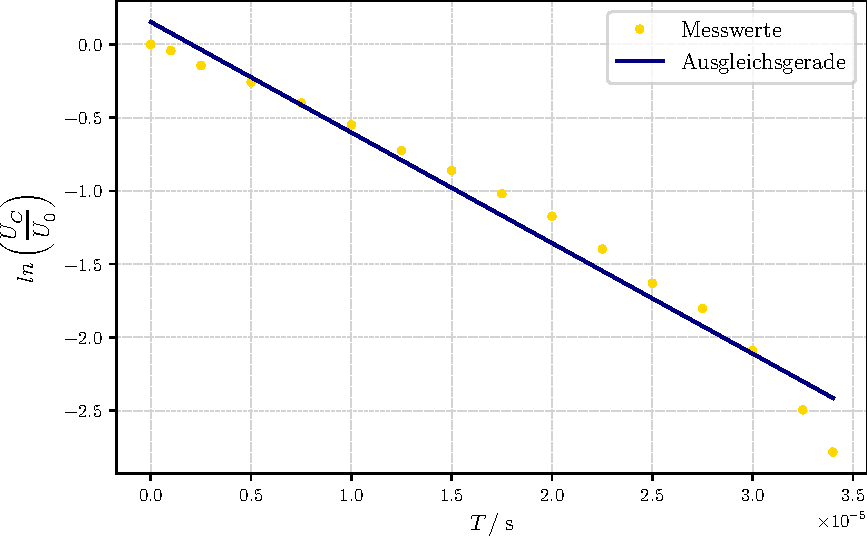
\includegraphics[width=\textwidth]{plot1.pdf}
\end{figure}

\subsection{Gelbe Spektrallinie}
\label{sec:gelbe_Spektrallinie}
Die Messwerte sind in \autoref{tab:gelb} und die Ausgleichsgerade in \autoref{fig:gelb} zu finden.
\begin{table}
    \centering
    \caption{Messwerte für die gelbe Spektrallinie.}
    \label{tab:rot}
    \begin{tabular}{c c}
        \toprule
        $U_{\symup{B}} / \unit{\milli\volt}$ & $I / \unit{\nano\ampere}$ \\
        \midrule
         0 & 1.000 \\
        20 & 0.900 \\
        40 & 0.810 \\
        60 & 0.720 \\
        80 & 0.640 \\
       100 & 0.550 \\
       120 & 0.475 \\
       140 & 0.400 \\
       160 & 0.350 \\
       180 & 0.290 \\
       200 & 0.230 \\
       220 & 0.190 \\
       240 & 0.150 \\
       260 & 0.100 \\
       280 & 0.100 \\
       300 & 0.090 \\
       320 & 0.060 \\
       340 & 0.050 \\
       360 & 0.040 \\
       380 & 0.010 \\
       400 & 0.010 \\
       420 & 0.005 \\
       440 & 0.000 \\
        \bottomrule
    \end{tabular}
\end{table}

\begin{figure}
    \centering
    \label{fig:gelb}
    \caption{Photostrom in Abhängigkeit der Bremsspannung und Ausgleichsgerade für die gelbe Spektrallinie.}
    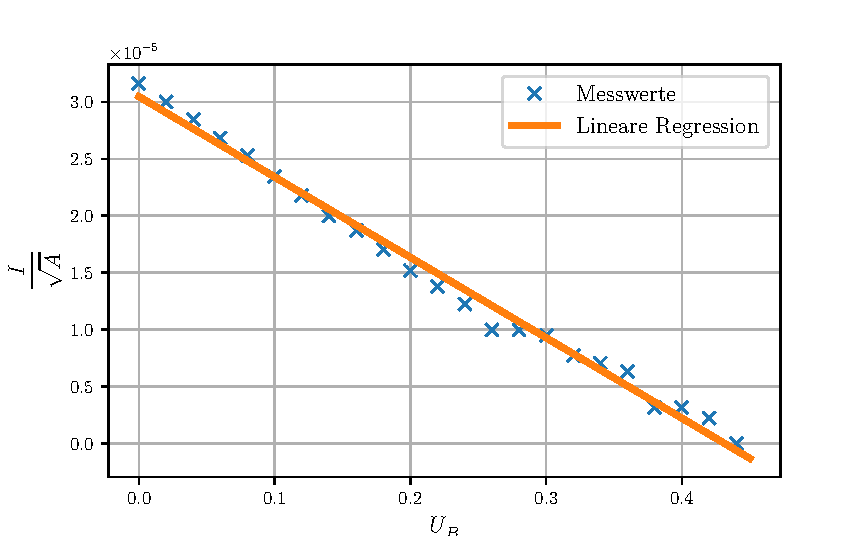
\includegraphics[width=\textwidth]{plot2.pdf}
\end{figure}